% $HeadURL$

%%%%%%%%%%%%%%%%%%%%%%%%%%%%%%%%%%%%%%%%%%%%%%%%%%%%%%%%%%%%%%%%%%%%%%
%%                     Association
%%%%%%%%%%%%%%%%%%%%%%%%%%%%%%%%%%%%%%%%%%%%%%%%%%%%%%%%%%%%%%%%%%%%%%

\subsection{Glyph: \glyph{Association}}\label{sec:association}

The association between one or more \glyph{EPNs} represents the non-covalent binding of the biological objects represented by those \glyph{EPNs} into a larger complex.

\begin{glyphDescription}
 \glyphSboTerm SBO:0000177 ! non-covalent binding.
 \glyphOrigin One or more \glyph{consumption} arcs (\sect{consumption}).
 \glyphTarget  One \glyph{production} arc (\sect{production}).
 \glyphNode An \glyph{association} between several entities is represented by a filled disc linked to two connectors, small arcs attached on point separated by 180 degrees. The consumption (\sect{consumption}) and production (\sect{production}) arcs are linked to the extremities of those connectors. 
 \end{glyphDescription}

\begin{figure}[H]
  \centering
  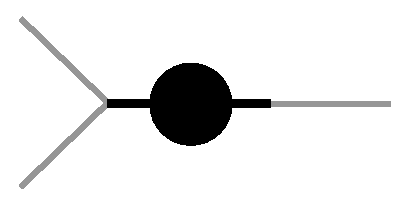
\includegraphics[scale = 0.5]{images/association}
  \caption{The \PD glyph for \glyph{association}.}
  \label{fig:association}
\end{figure}

The example in \fig{assoc-cyclin} illustrates the association of cyclin and CDC2 kinase into the Maturation Promoting Factor.

\begin{figure}[H]
  \centering
  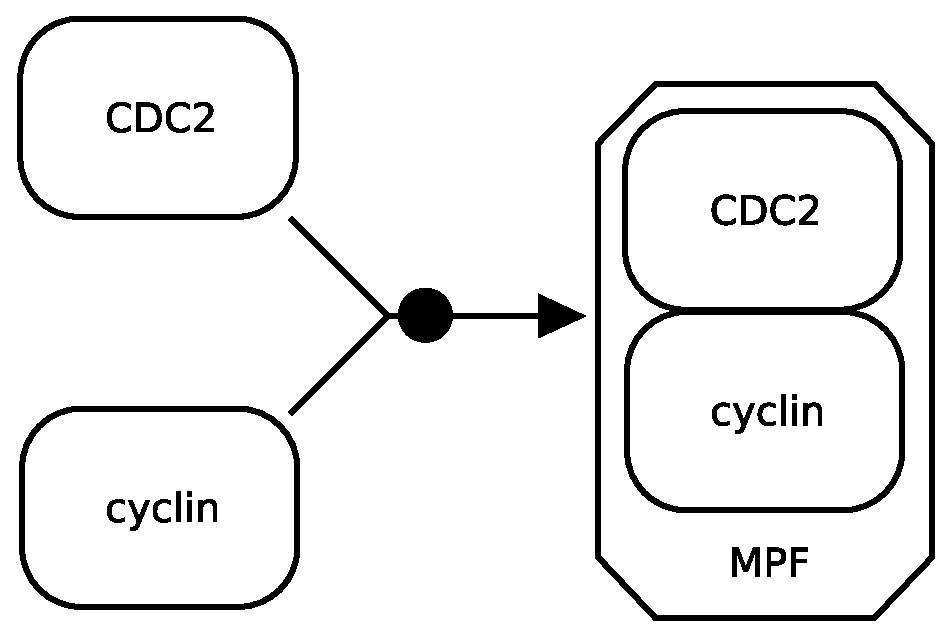
\includegraphics[scale = 0.3]{examples/association-MPF}
  \caption{Association of cyclin and CDC2 kinase into the Maturation Promoting Factor.}
  \label{fig:assoc-cyclin}
\end{figure}

\fig{assoc-unamed} gives an example illustrating the association of a pentameric macromolecule (a nicotinic acetylcholine receptor) with a simple chemical (the local anesthetic chlorpromazin) in an unnamed complex.

\begin{figure}[H]
  \centering
  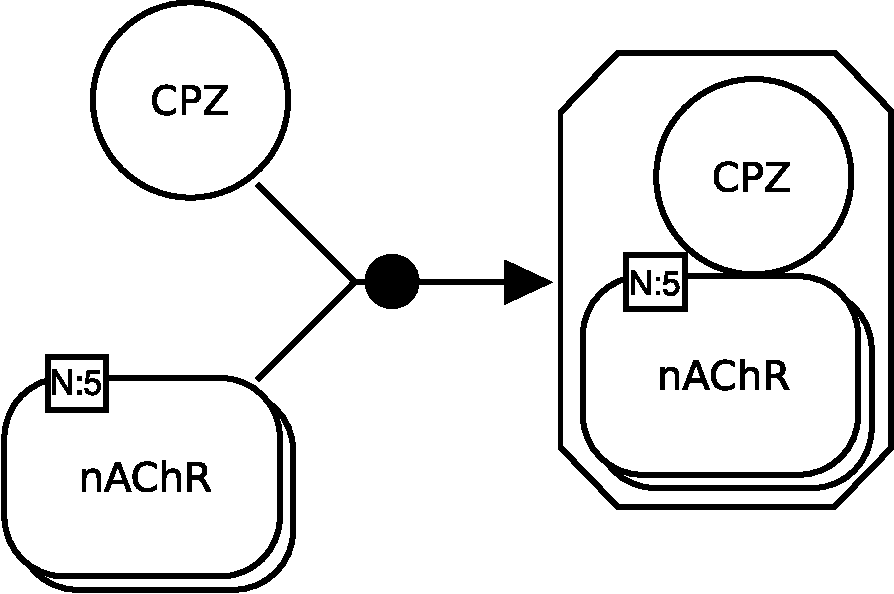
\includegraphics[scale = 0.3]{examples/association-unamed}
  \caption{The association of a pentameric macromolecule with a simple chemical in an unnamed complex.}
  \label{fig:assoc-unamed}
\end{figure}

An association does not necessarily result in the formation of a \glyph{complex}; it can also produce a \glyph{multimer}, or a \glyph{macromolecule} (although the latter case is semantically borderline).  \fig{assoc-multi} gives an example of this, using the formation of hemoglobin.

\begin{figure}[H]
  \centering
  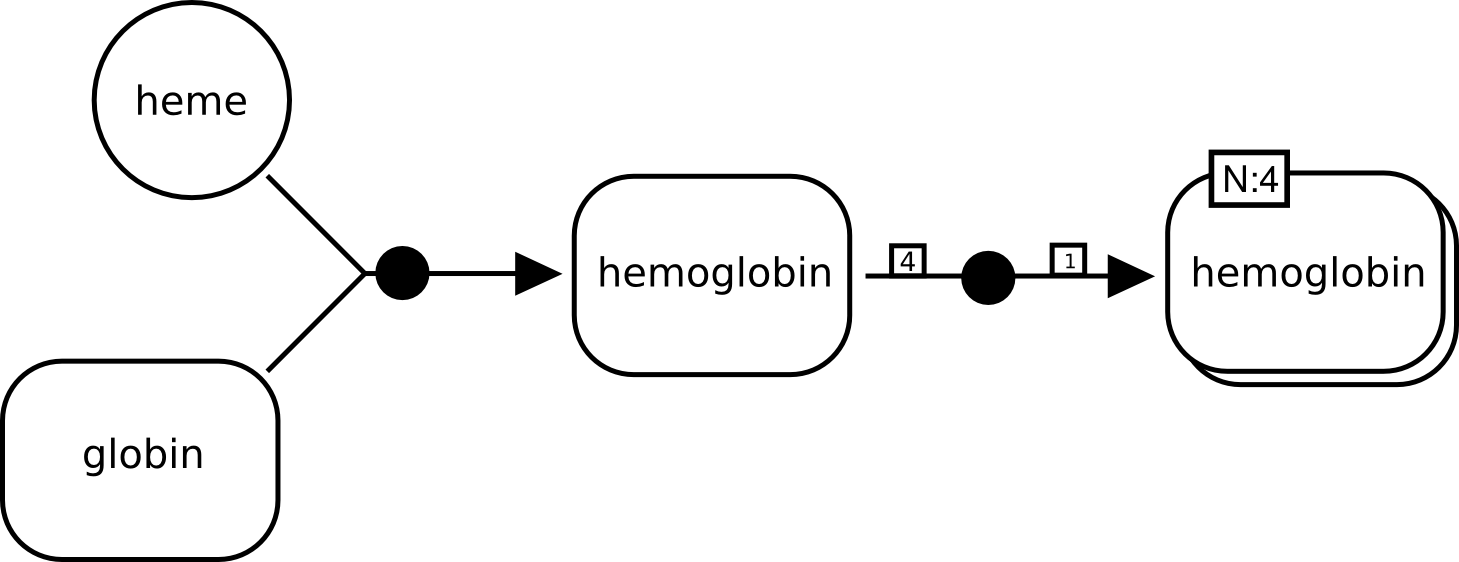
\includegraphics[scale = 0.3]{examples/association-multimerisation}
  \caption{Formation of hemoglobin.}
  \label{fig:assoc-multi}
\end{figure}



% The following is for [X]Emacs users.  Please leave in place.
% Local Variables:
% TeX-master: "../sbgn_PD-level1"
% End:
